\usepackage{../common}

\title{Feature set analysis for chess NNUE networks}
\subtitle{Tesis de Licenciatura}
\author{Martín Emiliano Lombardo}
\institute{Departamento de Computación\\Facultad de Ciencias Exactas y Naturales\\Universidad de Buenos Aires}
\date{2024}
\titlegraphic{
\includegraphics[height=1cm]{../assets/wN.pdf}}
\usetheme{Berlin}

%gets rid of bottom navigation bars
\setbeamertemplate{footline}[frame number]{}
%gets rid of bottom navigation symbols
\setbeamertemplate{navigation symbols}{}
%gets rid of footer
\setbeamertemplate{footline}{}

\begin{document}

\frame{\titlepage}

\section{Parte 1}

\subsection{Pepe}

\begin{frame}
\frametitle{Sample frame title}
This is some text in the first frame.\pause This is some text in the first frame. This is some text in the first frame.
\end{frame}

\begin{frame}
\frametitle{Sample frame title}

\begin{figure}[H]
\centering
\makebox[\textwidth]{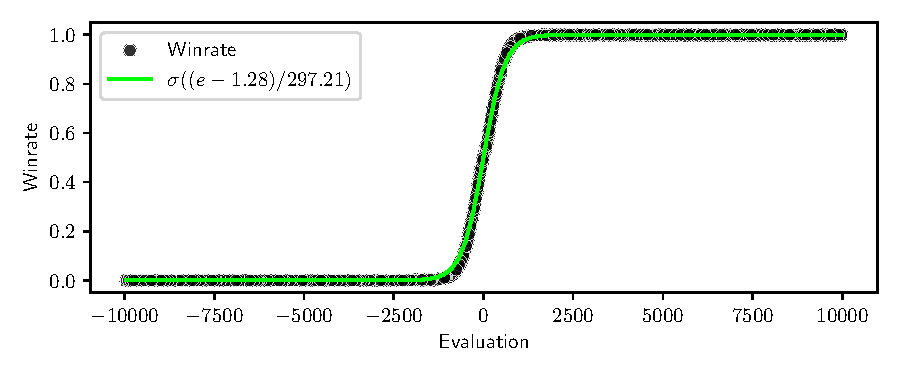
\includegraphics[width=\textwidth]{../assets/sigmoid_fit.pdf}}
\caption{WDL model function (sigmoid) fitted to 100 million evaluations in the dataset.}
\label{wdl-fit}
\end{figure}

\end{frame}

\section{Parte 2}

\begin{frame}
\frametitle{Sample frame title}

\begin{figure}[H]
\centering
\makebox[\textwidth]{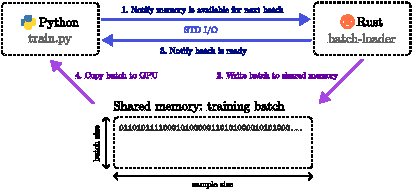
\includegraphics[width=\textwidth]{../assets/training-loop.pdf}}
\caption{Sequence of steps to send a batch from the \texttt{batch-loader} subprocess in Rust to Pytorch.}
\label{training-loop}
\end{figure}
\end{frame}

\end{document}
